\documentclass[a4paper,10pt]{article}
\usepackage[utf8]{inputenc}
\usepackage{hyperref}
\usepackage{cleveref}
\usepackage{tikz}
\usetikzlibrary{calc}
\usetikzlibrary{decorations.pathreplacing}
\usetikzlibrary{arrows, shapes, shadows, positioning}
\usepackage{pgf-umlcd}
\usepackage{amsmath}
\usepackage{textcomp}
\usepackage{caption}
\usepackage{framed}
\usepackage{graphicx}
\usepackage[margin=1.25in]{geometry}
\DeclareMathOperator*{\argmax}{arg\,max}
\DeclareMathOperator*{\arctanh}{arc\,tanh}
\usepackage{algorithm}
\usepackage{algorithmicx}
\usepackage{algpseudocode}
\usepackage{rotating}
\usepackage{url}
\usepackage{verbatim}
\usepackage[T1]{fontenc}


\title{LDPC Codes, Construction and Applications}
\author{Manu T S}

\begin{document}

\maketitle

\begin{abstract}
In this report we study construction of LDPC codes and implementation of encoder and decoder for LDPC codes. We implement the progressive edge growth algorithm,
algorith for construction of LDPC codes based on Reed-Solomon Codes. We also implement an encoder for LDPC codes. For decoder belief propogation decoder is 
implemented.
\end{abstract}

\section{Motivation}
\label{motivation}
Coding Theory is one of the foundations of Communication Engineering.
Search for better and better codes has always been an area of intense research.
For a long time there was a significant gap between the theoretical capacity and practically achievable capacity.
It is proved that LDPC codes introduced by Gallager, form a class of capacity approaching codes.
The research in that area was dormant for a long time till they were rediscovered in the late 1990s\cite{kay}.
It is shown that these codes decoded with iterative decoding algorithms like sum-product algorithm\cite{kay} or 
message passing algorithms\cite{mct} achieve good error performance.

GNU Radio provides a free and open-source platform for implementing practical communication systems 
using various compatible hardware like USRP, and also provides a learning and simulation tool.
The use of GNU Radio in research related to Software Defined Radio, Digital Signal Processing
and Communication Engineering is becoming increasingly widespread.
In this project we implement a generic encoder and decoder for LDPC codes in GNU Radio and
also implement algorithms for construction of LDPC codes.
\section{LDPC Codes}
The LDPC codes, as the name suggests is characterized by a sparse parity check matrix \textbf{H}.
From parity check matrix we can construct the \textit{Tanner graph} of the code. For example
\cref{tanner_example} represents the Tanner graph of [7, 4, 3] Hamming code with
\begin{equation}
\label{H_matrix}
 \textbf{H} = 
 \left(
\begin{array}{ccccccc}
1 & 1 & 0 & 1 & 1 & 0 & 0  \\
1 & 0 & 1 & 1 & 0 & 1 & 0  \\
0 & 1 & 1 & 1 & 0 & 0 & 1 
\end{array}
\right)
\end{equation}
A codeword \textbf{x} from the codebook described by parity check matrix \textbf{H} should satisfy
\begin{equation}
\label{parity_check_equations}
 \textbf{H}\textbf{x} = \textbf{0}
\end{equation}
In the Tanner graph of a $(t_c, t_r)$ regular binary LDPC code, each variable node will have degree $t_c$ 
and each check node will have degree $t_r$. Irregular LDPC codes can have different degrees for nodes.
Let $\lambda$ and $\rho$ be vectors such that their $i^{th}$ component $\lambda_i$ and $\rho_i$ represent the fraction of edges
connecting to a variable node of degree $i$ and check node of degree $i$ respectively.
Thus
\begin{equation}\nonumber
\lambda(x) = \displaystyle \sum_i \lambda_ix^{i-1} \hspace{8pt}\text{and}\hspace{8pt} \rho(x) = \displaystyle \sum_i \rho_ix^{i-1}
\end{equation}
are called variable and check degree distribution polynomials respectively.
Standard ensemble LDPC$(n, \lambda, \rho)$ of bipartite graphs is defined as the set of bipartite graphs with
$n$ variable nodes, variable degree distribution $\lambda(x)$ and check degree distribution $\rho(x)$.
%===========================================================================================================================
\begin{figure}
\begin{center}
\begin{tikzpicture}[var node/.style={scale = 0.8, circle,fill=blue!20,draw,font=\sffamily\Large\bfseries}, fun node/.style={scale = 0.8, circle,fill=yellow!20,draw,font=\sffamily\Large\bfseries}]
  \node[var node] (x7) at (0, 0) {$x_7$};
  \node[var node] (x6) at (0, -1) {$x_6$};
  \node[var node] (x5) at (0, -2) {$x_5$};
  \node[var node] (x4) at (0, -3) {$x_4$};
  \node[var node] (x3) at (0, -4) {$x_3$};
  \node[var node] (x2) at (0, -5) {$x_2$};
  \node[var node] (x1) at (0, -6) {$x_1$};  
  \node[fun node] (f3) at (4, 0) {$f_3$};
  \node[fun node] (f2) at (4, -3) {$f_2$};
  \node[fun node] (f1) at (4, -6) {$f_1$};
  \draw[thick,draw=gray!100] (x1) -- node [below = 6pt] {(a)} (f1);
  \draw[thick,draw=gray!100] (x2) --  (f1);
  \draw[thick,draw=gray!100] (x4) --  (f1);
  \draw[thick,draw=gray!100] (x5) --  (f1);
  \draw[thick,draw=gray!100] (x1) --  (f2);
  \draw[thick,draw=gray!100] (x3) --  (f2);
  \draw[thick,draw=gray!100] (x4) --  (f2);
  \draw[thick,draw=gray!100] (x6) --  (f2);
  \draw[thick,draw=gray!100] (x3) --  (f3);
  \draw[thick,draw=gray!100] (x2) --  (f3);
  \draw[thick,draw=gray!100] (x4) --  (f3);
  \draw[thick,draw=gray!100] (x7) --  (f3);
\end{tikzpicture}
\caption{\scriptsize{Tanner graph of [7, 4, 3] Hamming code with \textbf{H} given in \cref{H_matrix}.
The blue nodes on the left represents the components of a codeword. They are called variable nodes.
The yellow nodes on the right represents each of the constraints in the system \cref{parity_check_equations}. They are called
check nodes. When $h_{i,j}$ is 1 there exists a link between $j^{th}$ variable node and $i^{th}$ check node.
}} 
\label{tanner_example}
\end{center}
\end{figure}
\section{Marginalization Via Message Passing}
Consider a function $f$ with factorization:
\begin{align}
\ f(x_1,x_2,x_3,x_4,x_5,x_6)=f_1(x_1,x_2,x_3)f_2(x_1,x_4,x_6)f_3(x_4)f_4(x_4, x_5)
\end{align}
Now, the marginal of function $f$ w.r.t $x_1$ is:
\begin{eqnarray}
f(x_1) 	&=&\sum_{x_2, x_3, x_4, x_5, x_6} f(x_1,x_2,x_3,x_4,x_5,x_6) \\
	&=&\left[\sum_{x_2, x_3} f_1(x_1, x_2, x_3)\right]\left[\sum_{x_4}f_3(x_4)\left(\sum_{x_6}f_2(x_1, x_4, x_6)\right)\left(\sum_{x_5}f_4(x_4, x_5)\right)\right]
%f(x_1) &=&\sum_{x_2,x_4}f_1(x_1,x_2,x_4)\,\sum_{x_3,x_6}f_2(x_3,x_4,x_6)\,\sum_{x_5,x_7}f_3(x_4,x_5,x_7)
\end{eqnarray}
Factor graph associated with above factorization is given in Figure~\ref{fig:map0}. 
\begin{figure}[htbp]
\begin{center}
\begin{tikzpicture}[scale=1]
 \tikzstyle{cnode}=[rectangle, inner sep = 2pt, fill]
 \tikzstyle{vnode}=[circle, inner sep = 2pt, fill]
% \draw[color=red] (0,-2) node[vnode] (x2) {}; 
% \draw (-0.7, -2) node{$x_2$};
\draw [color=red](2,-2) node[vnode] (x1) {};
\draw (1.7, -2) node{$x_1$};
\draw [color=red](0,-4) node[vnode] (x2) {};
\draw (-0.3, -4) node{$x_2$};
\draw[color=red] (1,-4) node[vnode] (x3) {};
\draw (0.7, -4) node{$x_3$};
\draw[color=red] (2,-4) node[vnode] (x4) {};
\draw (1.7, -4) node{$x_4$};
\draw[color=blue] (2,-5) node[cnode] (f3) {};
\draw (1.7, -5) node{$f_3$};
\draw[color=blue] (3,-5) node[cnode] (f4) {};
\draw (2.7, -5) node{$f_4$};
\draw[color=red] (4,-4) node[vnode] (x6) {};
\draw (3.7, -4 ) node{$x_6$};
\draw[color=red] (3,-6) node[vnode] (x5) {};
\draw (2.7, -6) node{$x_5$};
\draw[color=blue] (1,-3) node[cnode] (f1) {};
\draw (0.7, -3) node{$f_1$};
\draw[color=blue] (3,-3) node[cnode] (f2) {};
\draw (2.7, -3) node{$f_2$};
\draw (x1) -- (f1);
\draw (x1) -- (f2);
\draw (f1) -- (x2);
\draw (f1) -- (x3);
\draw (f2) -- (x4);
\draw (f2) -- (x6);
\draw (x4) -- (f3);
\draw (f4) -- (x5);
\draw (x4) -- (f4);
\end{tikzpicture}
\end{center}
\caption{Factor Graph \label{fig:map0}}
\end{figure}
Here the red circles represent the variables ($x_1,x_2,\cdots,x_6$) and are called the \textit{variable-nodes}. Blue circles represent the factor ($f_1$,$f_2$,$f_3$ and $f_4$) 
and referred as the \textit{check-nodes}. In the factor graph, a variable-node is connected to a check-node iff the corresponding variable takes part in that factor.
Notice that this factor graph is a tree (i.e. there is no cycle in the graph). In the case where the factor graph is a tree the marginalization problem can be broken into smaller
tasks according to the structure of the tree. The algorithm is explained in the next paragraph

The alogorithm proceeds by sending messages along the edges of the tree. Messages are functions on $\mathcal{X}$, or equivalently, vectors of length $\left|\mathcal{X}\right|$.
The messages signify marginals of parts of the function and these parts are combined to form the marginal of the whole function. Message passing originates at the leaf nodes.
Messages are passed up the tree and as soon as a node has received messages from all its children, the incoming messages are processed and the result is passed up to the parent node.
Figure~\ref{fig:rules} explains the computation to be performed at the nodes during marginalization.

\begin{figure}[htbp]
\begin{center}
\begin{tikzpicture}[scale=1]
 \tikzstyle{cnode}=[rectangle, inner sep = 2pt, fill]
 \tikzstyle{vnode}=[circle, inner sep = 2pt, fill]
 \tikzstyle{line} = [draw, -latex']
 
 \begin{scope}
 \begin{scope}[xshift=-3cm]
    \draw[color=red] (0, 0) node[vnode] (x) {};
    \draw (0, 0.3) node{$x$};
    \draw[color=blue] (0,-1) node[cnode] (f) {};
    \draw (0, -1.3) node{$f$};
    \path [line] (f) -- node[left]{$\mu(x) = f(x)$} (x);
 \end{scope}

 \begin{scope}
  \draw (0, -0.30) node{initialization at};
  \draw (0, -0.70) node{leaf nodes};
 \end{scope}

 \begin{scope}[xshift=3cm]
    \draw[color=blue] (0, 0) node[cnode] (f) {};
    \draw (0, 0.3) node{$f$};
    \draw[color=red] (0,-1) node[vnode] (x) {};
    \draw (0, -1.3) node{$x$};
    \path [line] (x) -- node[right]{$\mu(x) = 1$} (f);  
  \end{scope}
  \end{scope}

  \begin{scope}[yshift=-3cm]
  \begin{scope}[xshift=-3cm]
 \draw[color=blue] (0, 0) node[cnode] (f) {};
 \draw (0.3, 0) node{$f$};
 \draw (0, 0.5) node{$\mu(x) = \prod_{k=1}^{K} \mu_k(x)$};
 \draw[color=red] (0,-1) node[vnode] (x) {};
 \draw (-0.3, -1) node{$x$};
 \draw[color=blue] (-1, -2) node[cnode] (f1) {};
 \draw (-1, -2.3) node{$f_1$};
 \draw[color=blue] (0, -2) node[cnode] (fk) {};
 \draw (0, -2.3) node{$f_k$};
 \draw[color=blue] (1, -2) node[cnode] (fK) {};
 \draw (1, -2.3) node{$f_K$};
 \path [line] (x) -- (f);
 \path [line] (f1) -- node[near start, left]{$\mu_1$} (x);
 \path [line] (fk) -- node[near start, left]{$\mu_k$} (x);
 \path [line] (fK) -- node[near start, right]{$\mu_K$} (x);
  \end{scope}
  
  \begin{scope}
    \draw (0, -0.80) node{variable/check};
    \draw (0, -1.20) node{node processing}; 
  \end{scope}

  \begin{scope}[xshift=3cm]
 \draw[color=red] (0, 0) node[vnode] (x) {};
 \draw (0.3, 0) node{$x$};
 \draw (0, 0.5) node{$\mu(x) = \sum_{\sim x}f(x, x_1, \cdots, x_K)\prod_{k=1}^{K} \mu_k(x)$};
 \draw[color=blue] (0,-1) node[cnode] (f) {};
 \draw (-0.3, -1) node{$f$};
 \draw[color=red] (-1, -2) node[vnode] (x1) {};
 \draw (-1, -2.3) node{$x_1$};
 \draw[color=red] (0, -2) node[vnode] (xk) {};
 \draw (0, -2.3) node{$x_k$};
 \draw[color=red] (1, -2) node[cnode] (xK) {};
 \draw (1, -2.3) node{$x_K$};
 \path [line] (f) -- (x);
 \path [line] (x1) -- node[near start, left]{$\mu_1$} (f);
 \path [line] (xk) -- node[near start, left]{$\mu_k$} (f);
 \path [line] (xK) -- node[near start, right]{$\mu_K$} (f);
  \end{scope}
  \end{scope}
  
  \begin{scope}[yshift=-7cm]
 \draw[color=blue] (0, 0) node[cnode] (f) {};
 \draw (0.5, 0) node{$f_{K + 1}$};
 \draw (0, 0.5) node{marginalization};
 \draw[color=red] (0,-1) node[vnode] (x) {};
 \draw (-0.3, -1) node{$x$};
 \draw[color=blue] (-1, -2) node[cnode] (f1) {};
 \draw (-1, -2.3) node{$f_1$};
 \draw[color=blue] (0, -2) node[cnode] (fk) {};
 \draw (0, -2.3) node{$f_k$};
 \draw[color=blue] (1, -2) node[cnode] (fK) {};
 \draw (1, -2.3) node{$f_K$};
 \draw (-1.5, -1) node{$\prod_{k=1}^{K+1} \mu_k(x)$};
 \path [line] (f) -- node[right] {$\mu_{K + 1}$} (x);
 \path [line] (f1) -- node[near start, left]{$\mu_1$} (x);
 \path [line] (fk) -- node[near start, left]{$\mu_k$} (x);
 \path [line] (fK) -- node[near start, right]{$\mu_K$} (x);
  \end{scope}
  
\end{tikzpicture}
\end{center}
\caption{Message Passing Rules \label{fig:rules}}
\end{figure}
To compute tha marginal with respect to all the variables, one can consider for each variable, a tree rooted in this variable and execute single marginal message passing algorithm 
on each rooted tree. Here all the computations can be performed simultaneously on a single tree. Start at all leaf nodes and for every edge compute the outgoing message along this
edge as soon as you have the incoming messages along all other edges that connect to a given node.
\section{Decoding Via Message Passing}
For memoryless channel without feedback, bitwise maximum a posteriori (MAP) decoding of a codeword is given by~\cite{mct}:  
\begin{align}
\hat x_i( y) &= \text{arg} \max_{x_i}p_{X_{i}|Y}(x_{i}| y) \label{eq:1}\\
\ &= \text{arg} \max_{x_i}\sum_{\sim x_i}p_{X|Y}( x| y) \label{eq:2}\\
\ &= \text{arg} \max_{x_i}\sum_{\sim x_i}p_{Y|X}( y| x)p_{X}( x) \label{eq:3}\\
\ &= \text{arg} \max_{x_i}\sum_{\sim x_i}\prod_{j}p_{Y_j|X_j}(y_j|x_j)p_{X}( x)\label{eq:4}
%\ &= \text{arg} \max_{x_i}\sum_{\sim x_i}\prod_{j}p_{Y_j/X_j}(y_j/x_j)\mathbf{1}_{x\in C}
\end{align}
The notation $\sum_{\sim x_i}$ indicates that sum is over all components of $x$, except $x_i$. 
We obtain \eqref{eq:2} from \eqref{eq:1} by total probability rule. On application of Bayes's rule,
we obtain \eqref{eq:3} from \eqref{eq:2}.
Equation \eqref{eq:2} has very high computational complexity.
For a codeword of length $n$ and rate $R$, approximate computational complexity is $\mathrm{O} (2^{nR})$. 
The computational complexity can be reduced by factorizing the sequence probability. To this end, in equation\eqref{eq:4}, 
we use the fact that the channel is memoryless, without feedback. Furthermore, since all the input codewords are equiprobable,
\begin{align}
\hat x_i(y) = \text{arg} \max_{x_i}\sum_{\sim x_i}\prod_{j}p_{Y_j|X_j}(y_j|x_j)\mathbf{1}_{\left\lbrace x\in C\right\rbrace} \label{eq:5}
\end{align} 
Where $\mathbf{1}_{\left\lbrace x\in C\right\rbrace}$ is a code membership function for the codebook $C$. Code membership function $\mathbf{1}_{\left\lbrace x\in C\right\rbrace}$
has a factorized form, and this factorization is used in efficient decoding.

\subsection{Message Passing decoder for Binary Erasure Channel}
By the standard message-passing rules the initial messages are $(\mu_j(0), \mu_j(1)) = (p_{Y_j|X_j}(y_j|0),(p_{Y_j|X_j}(y_j|1))$. In the case of binary erasure channel, the messages are
either $(1-\epsilon, 0), (\epsilon, \epsilon), \text{ or } (0, 1-\epsilon)$ corresponding to 0, ? (erasure), or 1 respectively received from channel output.
In this case we can normalize the message to (1, 0), (1, 1) and (0, 1) correspondingly. Now the message processing rules are discussed. \\
\textbf{Claim :} \\
For BEC general message passing rules shown in Figure \ref{fig:rules} simplify to the following. At a variable node the outgoing message 
is an erasure if all incoming messages are erasures. Otherwise, since the channel never introduces errors, all non-erasure messages must agree and either be 0 or 1. In this case
the outgoing message is equal to this common value. At a check node the outgoing message is an erasure if anu of the incoming message is an erasure. Otherwise, if all the
incoming messages are either 0 or 1, then the outgoing message is the mod-2 sum of the incoming messages \\
\textbf{Proof :} \\
If all messages entering a variable node are from the set $\left\lbrace(1, 0), (1, 1)\right\rbrace$, then the outgoing message, which is equal to the component-wise
product of the incoming messages according to the general message-passing rules, is also from this set. Further, it is equal to (1, 1) only if all incoming messages are 
of the form (1, 1) i.e, erasures. The equivalent statement is true if all incoming messages are from the set $\left\lbrace(1, 0), (1, 1)\right\rbrace$. Since channel never 
introduces errors, we only need to consider these two cases.
\section{Construction of the parity check matrix using Reed-Solomon code}\label{chap:"RS"}

The parity check matrix of a LDPC code is a sparse matrix. Ideally the Bipartite graph constructed using the  parity check matrix should not contain a 
cycle (no feedback) for optimal decoding. However, in practice it is hard to generate parity check matrices without cycles. Nevertheless most well 
defined methods for generating LDPC codes try to avoid cycles of length less than some minimum length (
minimum length could be any of the even positive integer like $6$, $8$, $10$, etc.). In this chapter we will discuss LDPC code construction based on 
Reed-Solomon codes\cite{IEEE1}, also known as RS-LDPC codes. The bipartite graph for these codes does not have cycle of length 4. 
A $(6,32)$ regular $(2048,1723)$ RS-LDPC code has been adopted as the FEC in the IEEE $802.3$an $10$GBase-T standard\cite{IEEE}. 

\subsection{Reed-Solomon codes} 

Consider the Galois field $GF(q)$ with $q$ elements, where $q$ is a positive integer power of a prime number. Let $\rho$ be a positive integer 
such that $2 \leq \rho $<$ q$. The generator polynomial of cyclic $(n,k,d_{min})$ code $C$ is given by:
\begin{align}
\ g(X)&= (X-\alpha)(X-\alpha^2)\cdot\cdot\cdot(X-\alpha^{\rho-2})\\
\ &= g_0+g_1X+\cdot\cdot\cdot+X^{\rho-2}
\end{align} 

Notice that $n=q-1$, $k=q-\rho+1$, $g_i\in GF(q)$ and $\alpha$ is a primitive element of a field. The parity check matrix $R_H$ for a 
Reed-Solomon code has size  $(\rho -2) \times n$. Any submatrix of size $(\rho -2)\times(\rho -2)$ of parity check matrix is the Vandermonde matrix. 
Therefore linear combination of any $(\rho -2)$ column will not result in $0_v$. The rank of matrix $R_H$ can be utmost $(\rho -2)$. Thus minimum distance is $d_{min}=(\rho -1)$. 

Now consider the $(q-1)$-tuple vector $g^{(0)}=(g_0,g_1,...,g_{\rho-2},0,0,...,0)$. Notice that $g_{\rho-2}=1$. By cyclically shifting $g^{(0)}$, we get generator 
matrix $G$ of size $k\times n$ for code $C$.
\[ G= \left( \begin{array}{cccccccccc}
g_0 & g_1 & g_2 & . & . & 1 & 0 & . & . & 0\\
0 & g_0 & g_1 & g_2 & . & . & 1 & .0 & . & . \\
\vdots & \vdots & \vdots & \vdots & \vdots & \vdots & \vdots & \vdots & \vdots & \vdots\\
0 & . & . & g_0 & g_1 & g_2 & . & . & . & 1 \end{array} \right)\] 

The generator matrix for shortened RS code $C_b$ is a submatrix of size $2 \times \rho$ and it is shown below:
\begin{align*}
 G_b= \begin{pmatrix}
g_0 & g_1 & g_2 & . & . & . & 1 & 0\\
0 & g_0 & g_1 & g_2 & . & . & . &1 \end{pmatrix}
\end{align*} 

\subsection{Properties of $C_b$} 
\begin{enumerate}
\item Since the length of codewords in $C_b$ is $\rho$ and the minimum distance between two codewords of $C_b$ is $(\rho-1)$, two codewords in $C_b$ only agree at most at one location.
\item Let $c$ be a codeword of weight $\rho$. If we multiply $c$ by $\forall \beta \in GF(q)$, we get set $C_b^{(1)}$ of $(q-1)$ codewords of weight $\rho$. 
    Now, length of every codeword of $C_b^{(1)}$ is also $\rho$. So $C_b^{(1)}$ is a MDS (Maximum Distance Separable) code.
\item Let us partition $C_b$ into a $q$ cosets $C_b^{(1)},C_b^{(2)},...,C_b^{(q)}$ based on $C_b^{(1)}$. Notice that $C_b^{(i)}$ is MDS code. 
    Therefore two codewords in any coset $C_b^{(i)}$ must differ in all the locations. 
\end{enumerate}

\subsection{Construction}
Let us now explain the explicit construction procedure for a LDPC code check matrix $H$.
\begin{enumerate}
\item All $q$ elements of $GF(q)$ can be expressed as some power of a primitive element $\alpha$. Let us define the location vector of $\alpha^i$ as a $q$-tuple over $GF(2)$, $$z(\alpha^i)=(0,0,...,1,0,...,0)$$, where $i^{th}$ element of $z(\alpha^i)$ is $1$ and all other elements are $0$. Choose one codeword $b=(b_1,b_2,...,b_{\rho}) \in C_b^{(i)}$. If we replace each $b_i$ ($1 \leq i \leq \rho $) by its location vector $z(b_i)$, we get a $z(b)=(z(b_1),z(b_2),...,z(b_{\rho}))$, which is a $ \rho q$-tuple of weight $\rho$ over $GF(2)$.
\item Arrange all $q$ $\rho q$-tuple of $C_b^{(i)}$ as rows of a matrix and call this matrix as $A_i$. The weight of each column of $A_i$ is $1$. 
\item Choose a positive integer $\gamma$, such that $1 \leq \gamma \leq q$. Then the parity check matrix $H$ of size $\gamma q \times \rho q$ is defined as:
\begin{align}
 H \overset{\triangle}{=}  \begin{bmatrix}
A_1\\
A_2\\
\vdots\\
A_{\gamma} \end{bmatrix} 
\end{align}
\end{enumerate}
Since each column of $A_i$ has weight $1$, weight of an each column of $H$ is $\gamma$. So, $H$ is a $(\gamma , \rho)$-regular matrix. Each row in $A_i$ is a coset member, so each row in $A_i$ is different,
\begin{enumerate}
\item Two rows in $A_i$ do not have single common element, 
\item Two codewords in $C_b$ agree at at most one symbol location ($d_{min}=\rho-1$). 
\end{enumerate}
From Property~$1$ and $2$ above, no two rows from $A_i,~A_j,~i\neq j$ agree at more than a single element. This will imply that the bipartite graph corresponding to $H$ is free of length 4 cycles. To see this, notice that our construction guarantees a $H$ which contains no rectangle having all the corner points non-zero. 

In this chapter we have shown the construction of a ($\gamma,\rho$) regular RS-LDPC. This code has girth at least six. In the next chapter we show the construction of an irregular LDPC code.
\section{Construction of Parity Check Matrix using Progressive Edge Growth}
In this section, we present progressive edge growth (PEG) method for the construction of regular and irregular LDPC code. 
A bipartite graph can be described using bit nodes, check nodes and set of edges $E$. In this method, edges between bit nodes and check nodes are 
established in a progressive manner. For given bit node, an edge connects the one of the check node such that girth is maximum. 
Thus, PEG algorithm has large girth when compared to codes constructed using random methods. 
Hence, code constructed using PEG algorithm has low error floor in comparison with code constructed using random methods.

Let us describe bit node degree sequence as follow:
\begin{equation*}
 D_b=\{{d_b}_1,{d_b}_2,\cdots,{d_b}_n\},~ {d_b}_1 \leq {d_b}_2 \leq \cdots \leq {d_b}_n
\end{equation*}
%
Where ${d_b}_i$ presents the degree of $i^{th}$ bit node.

\begin{algorithm}[H]
\caption{Progressive Edge Growth Algorithm\cite{peg}}
\label{peg_algo}
%\algsetup{indent=2em}
\begin{algorithmic}[1]
\State \textbf{Input:} sequence $D_b$
\State \textbf{Output:} parity check matrix $H$
\State initialize all check nodes with degree $0$
\For{$i=1$ to $n$}
\For{$j=1$ to ${d_b}_i$}
\If{$j=1$}
\State $1.~$find minimum degree check nodes set $C=\{c_1,c_2,\cdots,c_m\},~ 1 \leq m\leq n-k$ such that $deg(c_1)=deg(c_2)=\cdots=deg(c_m)$
\State $2.~$choose check node $c_1 \in C$
\State $3.~$put an edge between $i^{th}$ bit node and check node $c_1$
\State $4.~$increase the degree of $c_1$ by 1
\Else
\State $1.~$for $i^{th}$ bit node find check nodes set $C=\{c_1,c_2,\cdots,c_m\},~1\leq m\leq n-k$ such that girth is maximum and $deg(c_1) \leq deg(c_2) \leq \cdots \leq deg(c_m)$
\State $2.~$put an edge between $i^{th}$ bit node and check node $c_1$ 
\State $3.~$increase the degree of $c_1$ by 1
\EndIf
\EndFor
\EndFor
\end{algorithmic}
\end{algorithm}
%
Check node degree distribution obtained using Algorithm \ref{peg_algo} is almost uniform. Whenever multiple choices are available to 
pick check node from set $C$, we can either pick first check node in the set $C$ or pick any check node from set $C$. 
In algorithm \ref{peg_algo}, we always choose the first member of set $C$.
 \section{Encoding}
 If the parity check matrix is given as $\mathbf{\left[{I \; P}\right]}$, where $\mathbf{I}$ is $N - K$ x $N - K$ identity matrix, $\mathbf{P}$ is some $N - K$ x $K$ matrix,
   a codeword $\mathbf{x = \left[x_p^{\mathsf{T}} \; x_d^{\mathsf{T}}\right]^{\mathsf{T}}}$ can be formed by assigning
    \begin{equation}\nonumber
    \mathbf{x_p = P \cdot x_d}
    \end{equation}
   We obtain $\mathbf{G = \left[{I \; P}\right]}$ from $\mathbf{H}$ by Column permutation, Row additions and Row permutations
   Suppose $f$ represents the permutation in obtaining $\mathbf{G}$ from $\mathbf{H}$, and $\mathbf{G \cdot x = 0}$, then $\mathbf{H} \cdot f(\mathbf{x}) = \mathbf{0}$
      \begin{figure}[!htbp]
      \centering
    \begin{tikzpicture}
    \begin{scope}
      \foreach \c/\i [count=\n] in  
        {blue!20/$x_0$,blue!20/$x_1$,blue!20/$x_2$,red!20/$x_3$,red!20/$x_4$,red!20/$x_5$,red!20/$x_6$} 
           \node[draw,fill=\c,minimum height=0.75cm,minimum width = 1cm,xshift=\n*1cm](N\n){\i} ;
	    \draw [decoration={brace,raise=3pt},decorate] (N1.north west) --  node[above=10pt]{$\mathbf{x_p}$}(N3.north east); 
	    \draw [decoration={brace,raise=3pt},decorate] (N3.north east) --  node[above=10pt]{$\mathbf{x_d}$}(N7.north east);
	    \node[right of N1] {$\mathbf{x}$};
	    \coordinate (x0) at (1cm,-0.375cm);
	    \coordinate (x1) at (2cm,-0.375cm);
	    \coordinate (x2) at (3cm,-0.375cm);
	    \coordinate (x3) at (4cm,-0.375cm);
	    \coordinate (x4) at (5cm,-0.375cm);
	    \coordinate (x5) at (6cm,-0.375cm);
	    \coordinate (x6) at (7cm,-0.375cm);
	    \end{scope}
    \begin{scope}[yshift = -2cm]
      \foreach \c/\i [count=\n] in  
        {yellow!20/2,yellow!20/0,yellow!20/3,yellow!20/1,yellow!20/5,yellow!20/4,yellow!20/6} 
           \node[draw,fill=\c,minimum height=0.75cm,minimum width = 1cm,xshift=\n*1cm](N\n){\i} ;
           \node[right of N1] {$f$};
           \coordinate (p0a) at (1cm, +0.375cm);
           \coordinate (p0b) at (1cm, -0.375cm);
           \coordinate (p1a) at (2cm, +0.375cm);
           \coordinate (p1b) at (2cm, -0.375cm);
           \coordinate (p2a) at (3cm, +0.375cm);
           \coordinate (p2b) at (3cm, -0.375cm);
           \coordinate (p3a) at (4cm, +0.375cm);
           \coordinate (p3b) at (4cm, -0.375cm);
           \coordinate (p4a) at (5cm, +0.375cm);
           \coordinate (p4b) at (5cm, -0.375cm);
           \coordinate (p5a) at (6cm, +0.375cm);
           \coordinate (p5b) at (6cm, -0.375cm);
           \coordinate (p6a) at (7cm, +0.375cm);
           \coordinate (p6b) at (7cm, -0.375cm);
	    \end{scope}	    
    \begin{scope}[yshift = -4cm]
      \foreach \c/\i [count=\n] in  
        {blue!20/$x_1$,red!20/$x_3$,blue!20/$x_0$,blue!20/$x_2$,red!20/$x_5$,red!20/$x_4$,red!20/$x_6$} 
           \node[draw,fill=\c,minimum height=0.75cm,minimum width = 1cm,xshift=\n*1cm](N\n){\i} ;
            \node[right of N1] {$f\left(\mathbf{x}\right)$};
	    \coordinate (y0) at (3cm,+0.375cm);
	    \coordinate (y1) at (1cm,+0.375cm);
	    \coordinate (y2) at (4cm,+0.375cm);
	    \coordinate (y3) at (2cm,+0.375cm);
	    \coordinate (y4) at (6cm,+0.375cm);
	    \coordinate (y5) at (5cm,+0.375cm);
	    \coordinate (y6) at (7cm,+0.375cm);
	    \end{scope}	 
    \draw [->, thin, gray] (x0) -- (p0a);
    \draw [->, thin, gray] (p0b) -- (y0);
    \draw [->, thin, gray] (x1) -- (p1a);
    \draw [->, thin, gray] (p1b) -- (y1);
    \draw [->, thin, gray] (x2) -- (p2a);
    \draw [->, thin, gray] (p2b) -- (y2);
    \draw [->, thin, gray] (x3) -- (p3a);
    \draw [->, thin, gray] (p3b) -- (y3);
    \draw [->, thin, gray] (x4) -- (p4a);
    \draw [->, thin, gray] (p4b) -- (y4);
    \draw [->, thin, gray] (x5) -- (p5a);
    \draw [->, thin, gray] (p5b) -- (y5);
    \draw [->, thin, gray] (x6) -- (p6a);
    \draw [->, thin, gray] (p6b) -- (y6);
    \end{tikzpicture}
   \end{figure}


\begin{algorithm}[H]
\caption{Construction of $\mathbf{G = \left[{I \; P}\right]}$}
\label{encode_algo}
%\algsetup{indent=2em}
\begin{algorithmic}
\State \textbf{Input:} Parity Check matrix $\mathbf{H}$
\State \textbf{Output:} $\mathbf{G = \left[{I \; P}\right]}$
\State $nchk$ $\gets$ Number of rows of $\mathbf{H}$
\State $nvar$ $\gets$ Number of columns of $\mathbf{H}$
\State $limit$ $\gets$ Number of rows of $\mathbf{H}$
\State $rank$ $\gets$ 0
\State $i \gets$ 0
\State $f \gets (1, 2, 3, \dots, nvar)$
\While {$i < limit$} \Comment{Pivoting at (i, i)}
  \State $found \gets$ False \Comment{Flag indicating if the row contains non-zero entry}
  \For{$j$ from $i$ to $nvar$}
  \If{$\mathbf{H}[i, j] = 1$} \Comment{Encountering a non-zero entry at $(i, j)$}
  \State $found \gets $ True
  \State $rank \gets rank + 1$ \Comment{Increment rank}
  \State swap columns $i$ and $j$ \Comment{Now the entry at $(i, i)$ is 1}
  \State swap $f(i)$ and $f(j)$ \Comment{Keeping track of the column permutation}
  \State break
  \EndIf
  \EndFor
  \If{$found = $ true}
  \For {$k$ from $i$ to $nchk$}
  \If {$\mathbf{H}[k, i] = 1$} \Comment{Checking for non-zero entries below $(i, i)$}
  \State Add row $i^{th}$ row to $k^{th}$ row
  \EndIf
  \EndFor
  \EndIf
  \If{$found = $ false} \Comment{We encounter a row with all zeros}
  \For {$rows$ in $i$ to $limit$}
  \State swap row $rows$ with $rows + 1$ \Comment{Pushing the all-zero row to the bottom}
  \EndFor
  \State $limit \gets limit - 1$
  \EndIf
\EndWhile
\end{algorithmic}
\end{algorithm}
\section{Outcomes and Results}

Following classes and blocks were desingned as part of this project. These can be installed as an Out of Tree module in GNU Radio. The source can be downloaded from \cite{gr-ldpc}
   \begin{itemize}
    \item Class for GF$\left(2\right)$ Vector arithmetic.
    \item Class for GF$\left(2\right)$ Matrix arithmetic.
    \item Class for accessing LDPC codes in ``alist-file''\cite{alist} format.
    \item Class for holding an LDPC code.
    \item Class for message passing mechanisms for BSC and AWGN channels.
    \item LDPC Encoder block.
    \item LDPC Decoder blocks, for both float inputs and byte inputs.
    \item Two algorithms for construction of LDPC codes
   \end{itemize}

   Tables~\ref{tab:biter} and \ref{tab:blocker} compares the performance of these blocks with uncoded BPSK. The plot of Bit error performance is in Figure~\ref{fig:berplot}
   The GNU Radio set up used in this experiment is shown in Figure~\ref{fig:blocks}
   
\begin{table}
\caption{Bit Error Rate Comparison}\label{tab:biter}
\begin{center}
 \begin{tabular}{| c | c | c | c | c |}
 \hline
  sigma & Errors (No code)	& BER (No Code)	& Errors (With LDPC)	& BER (With LDPC) 	\\ \hline
  0.3  	& 4338			& 0.0004338	& 0			& 0			\\ \hline
  0.4	& 61814			& 0.0061814	& 0			& 0			\\ \hline
  0.5	& 227228		& 0.0227228	& 31			& 3.1e-06		\\ \hline
  0.6	& 477744		& 0.0477744	& 65855			& 0.0065855		\\ \hline
  0.7	& 765326		& 0.0765326	& 572393		& 0.0572393		\\ \hline
  0.8	& 1055848		& 0.1055848	& 968856		& 0.0968856		\\ \hline
  0.9	& 1332039		& 0.1332039	& 1291208		& 0.1291208		\\ \hline
  1.0	& 1585653		& 0.1585653	& 1565803		& 0.1565803		\\ \hline
 \end{tabular}
\end{center}
 \caption*{The performance of a (3, 6) regular LDPC code with $N = 96, K = 50,$ and $M = 48$}
\end{table}

\begin{table}
\caption{Block Error Rate Performance} \label{tab:blocker}
\begin{center}
 \begin{tabular}{| c | c | c | c | c |}
 \hline
  sigma & Errors (No Code)	& BER (No Code)	& Errors (With LDPC)	& BER (With LDPC) 	\\ \hline
  0.3  	& 3898			& 0.196461	& 0			& 0			\\ \hline
  0.4	& 18938			& 0.954488	& 0			& 0			\\ \hline
  0.5	& 19840			& 0.999994	& 0			& 0			\\ \hline
  0.6	& 19841			& 1.0		& 17			& 0.0008568		\\ \hline
  0.7	& 19841			& 1.0		& 19841			& 1.0			\\ \hline
 \end{tabular}
 \end{center}
 \caption*{The performance of an LDPC code generated using PEG with $N = 1008, K = 504,$ and $M = 504$}
\end{table}

  \begin{figure}
  \centering
   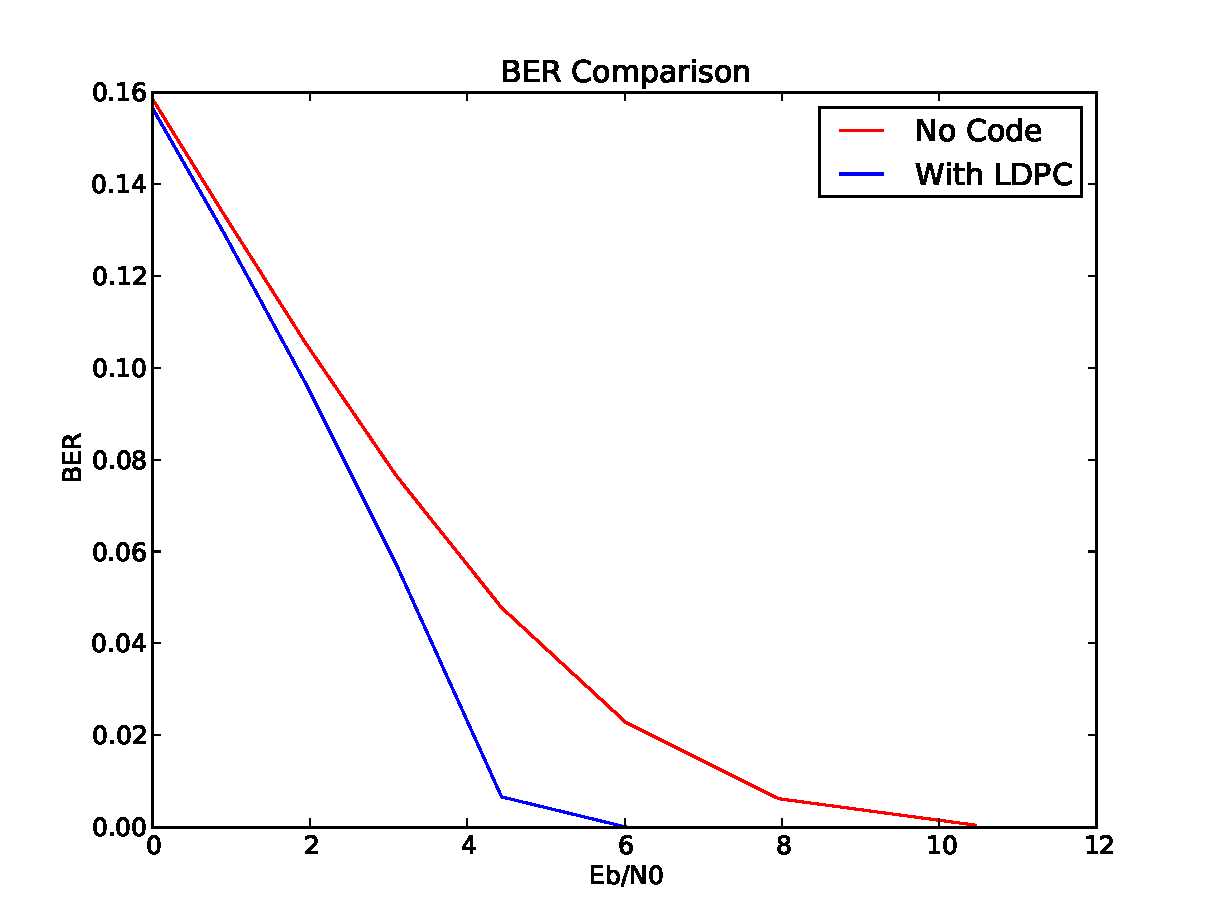
\includegraphics[scale = 0.5]{ber_plot.pdf}
   \caption{BER plot corresponging to Table~\ref{tab:biter}}
   \label{fig:berplot}
  \end{figure}

  \begin{figure}
  \centering
   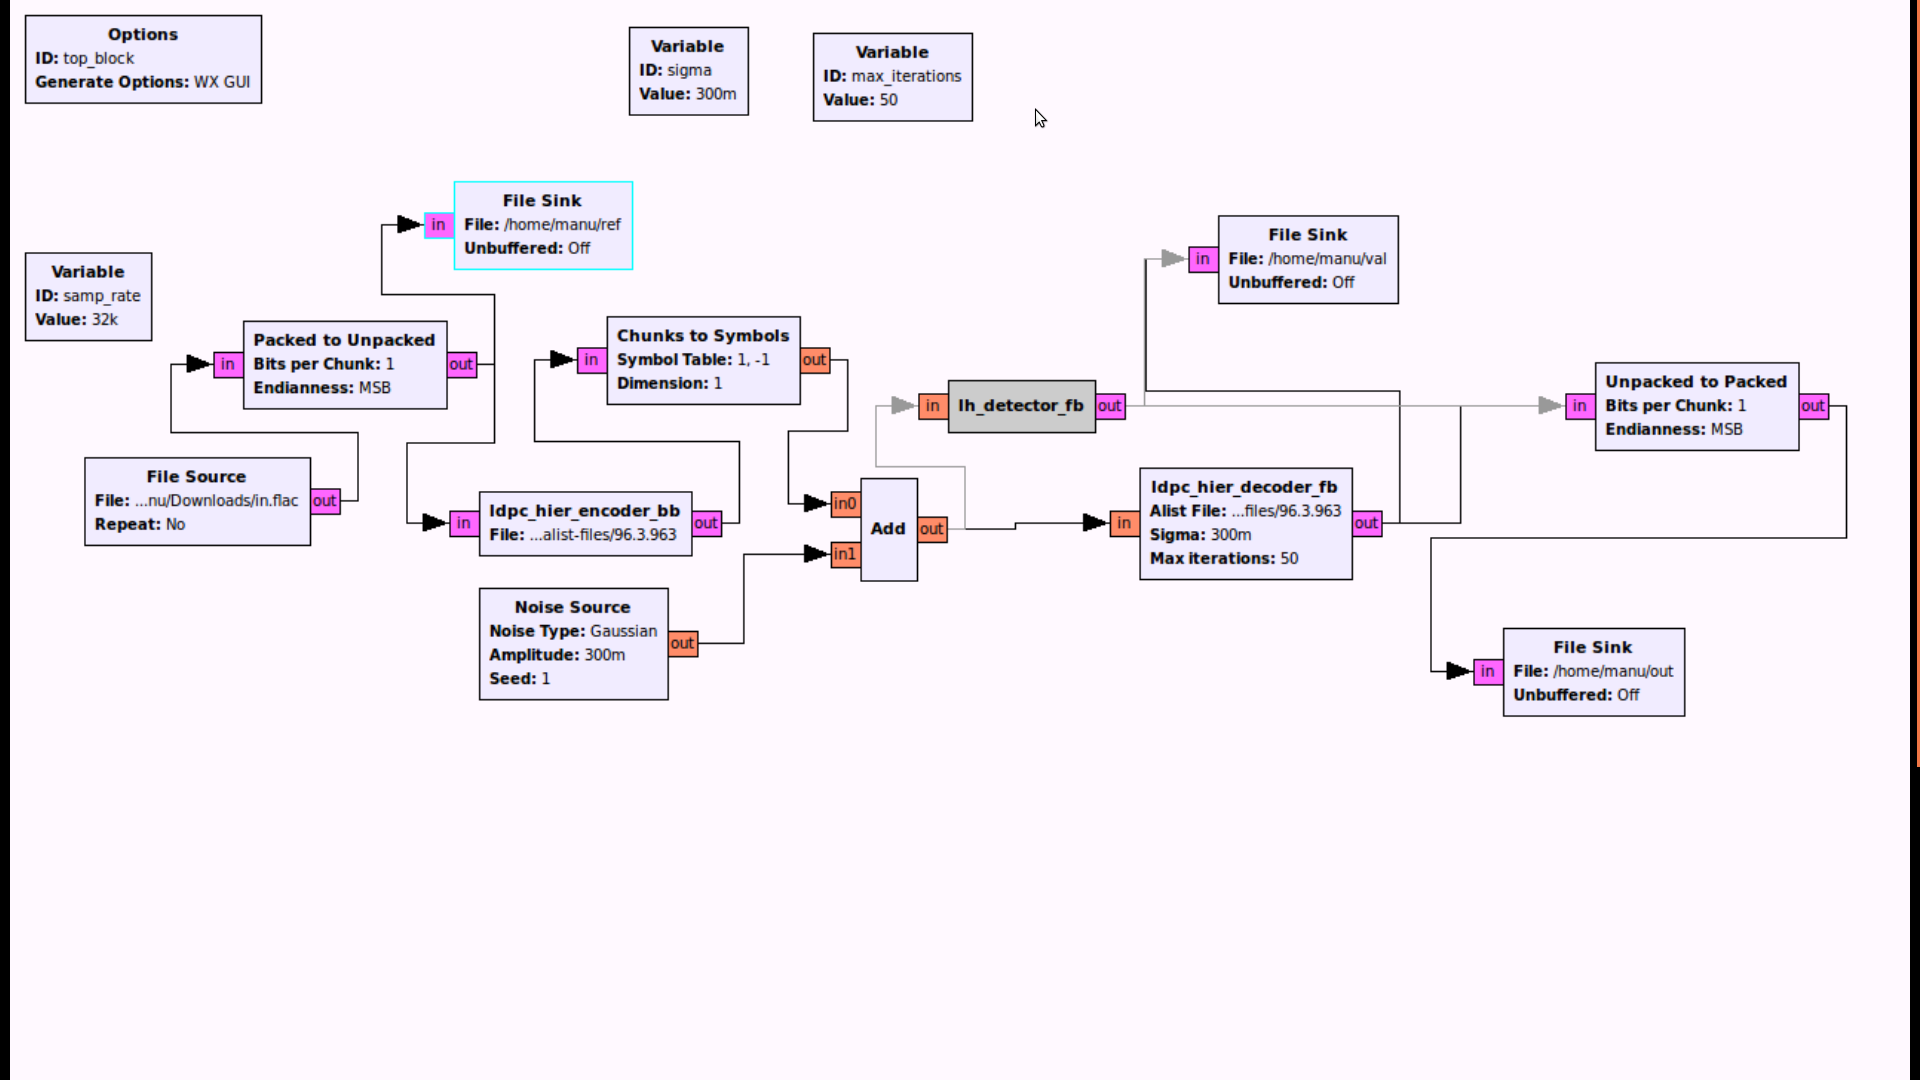
\includegraphics[scale = 0.2]{ldpc.png}
   \caption{GNU Radio block diagram} 
   \label{fig:blocks}
  \end{figure}
\clearpage
\begin{thebibliography}{9}

\bibitem{mct} T. Richardson and R. Urbanke, ``Modern Coding Theory'', Cambridge 2003.

\bibitem{rs_ldpc} I. Djurdjevic,  Jun Xu, K. Abdel-Ghaffar and Shu Lin, 
``A class of low-density parity-check codes constructed based on Reed-Solomon codes with two information symbols'',
IEEE Communication Letters, July 2003.

\bibitem{irrldpc} T. Richardson, M Amin Shokrollahi and R. Urbanke,``Design of Capacity Approaching Irregular 
Low-Density Parity-Check Codes'', Transactions On Information Theory, February 2001.

\bibitem{peg} Xiao-Yu Hu, Evangelos Eleftheriou and Dieter M. Arnold, ''Regular and Irregular Progressive Edge-Growth
Tanner Graphs'', Transactions on Information Theory, January 2005.

\bibitem{mask} Jun Xu, Lei Chen, I. Djurdjevic, Shu Lin and K. Abdel-Ghaffar, ``Construction of Regular and Irregular
LDPC codes: Geometry Decomposition and Masking'', Transactions on Information Theory, January 2007.

\bibitem{kay} David J. C. MacKay, ``Good Error-Correcting Codes Based on Very Sparse Matrices'', Transactions on Information
Theory, March 1999.

\bibitem{blahut} Richard E. Blahut, ``Algebraic Codes for Data Transmission'', Cambridge University Press 2003.

\bibitem{2user} Abdelaziz Amraoui, Sanket Dusad and R. Urbanke, ``Iterative Coding for Discrete-Time Multiple Access Channel''

\bibitem{sloane} F.J. MacWilliams and N.J.A. Sloane. ``Theory of Error-Correcting Codes'', North-Holland Publishing Company 1977. 

\bibitem{alist} \url{http://www.inference.phy.cam.ac.uk/mackay/codes/alist.html}

\bibitem{gr-ldpc} \url{https://github.com/manuts/gr-ldpc}
\end{thebibliography}

\end{document}